\documentclass[runningheads]{llncs}
%
\usepackage{subfig}
\usepackage{graphicx}
% Used for displaying a sample figure. If possible, figure files should
% be included in EPS format.
%
% If you use the hyperref package, please uncomment the following line
% to display URLs in blue roman font according to Springer's eBook style:
% \renewcommand\UrlFont{\color{blue}\rmfamily}

\begin{document}
%
\title{Automated environment modeling with drones}
%
%\titlerunning{Abbreviated paper title}
% If the paper title is too long for the running head, you can set
% an abbreviated paper title here
%
\author{Julian Bialas}
%

\institute{Fachhochschule Kufstein, Andreas Hofer-Straße 7, 6330 Kufstein, Austria} 

\maketitle              % typeset the header of the contribution
%
\begin{abstract}

This paper contains an evaluation of state of the art monocular vSLAM algorithms, that are suitable for 
autonomous exploration and mapping tasks for an unmanned aerial vehicle. Specifically, ORB- DSM- and DSO SLAM are examined concerning performance and effectiveness using the commonly used benchmark dataset EuRoC. With a difference to most similar evaluations \cite{point_cloud_eval}, in this paper the resulting point cloud is evaluated regarding density and accuracy, since the point cloud is crucial for a successful flight path navigation. A ROS framework is implemented, making it possible to easily combine the SLAM algorithm with a flight path algorithm within a simulated virtual environment. 

\keywords{vSLAM  \and Flight Path Planning \and Drones}
\end{abstract}
%
%
%
\section{Introduction}

Multiple applications exist for the autonomous exploration and mapping tasks for drones; such as search and rescue-, inspection- and surveillance operations \cite{tasks}. The focus of this paper is evaluating the feasibilty to perform an exploration and mapping task with a drone.
An approach with a combination of a vSLAM (visual simultaneous localization
and mapping) algorithm and a path planning algorithm is assessed. As the name 
suggests, the aim of a SLAM algorithm is to create a map of its completely unknown environment, while localizing itself within it only be using certain sensors. This paper is limited to monocular vSLAM, meaning that the algorithm is only working with a single RGB camera as a sensor. This makes the drone very affordable, making it highly available for a larger user group.  
The main part of this work is the evaluation of vSLAM algorithms in order to find the 
most suitable method, that meets the requirements for this autonomous navigation task. DSO (Direct Sparse Odometry) SLAM, DSM (Direct Sparce Mapping) SLAM and ORB (Oriented FAST and Rotated BRIEF) SLAM were investigated regarding accuracy of the resulting trajectory estimation and point cloud and computational speed. 
Furthermore, a ROS (Roboter Operating System) setup to combine the most suitable vSLAM algorithm with a flight path planning algorithm is introduced. This setup will be based on a simulated environment, making it easy to apply several different algorithms. Finally a recommendation for future work regarding 
the flight path algorithm is given.



\section{Methods}

After investigating common and suitable vSLAM algorithms for the autonomous
environment modeling task, these algorithms are evaluated regarding the 
quality of the computed trajectories, the accuracy and density of the predicted point clouds and the computational effectiveness by using the commonly used benchmark dataset EuRoC. 
The trajectories are aligned with the ground truth trajectories using the method of Umeyame \cite{ume}, visually
observed and the distances to the true position is evaluated. 
The point clouds are also aligned to the world reference of the ground truth point cloud, visually observed, and the distances to the closest point of 
the ground truth point cloud computed. Also the number of points predicted for 
each sequence in the dataset is taken into account. 
The computational time and resulting frames per second indicates the computational effectiveness. 
After a vSLAM algorithm with suitable attributes is exposed, it is 
implemented in a framework of a ROS environment, in order to apply 
flight planning algorithms in the future. 

\section{Intermediate results}

The results reflect the differences of the respective vSLAM algorithms.
Summarizing the results from the trajectory estimation by the algorithms, 
DSM and ORB both showed good results, with a positional error below 10cm 
for most sequences. DSO yields worse results, especially sequences that were
recorded in the vicon room (6/11).


As feature based algorithms usually estimate fewer points of the resulting 
point cloud \cite{point_cloud}, compared to DSM and DSO slam ORB-SLAM delivers fewer elements of the calculated point cloud. This can 
clearly be seen in figure \ref{fig:pointcloud}, where predicted points (red) are drawn into the ground truth points (white). However, 
ORB yields better results regarding the accuracy of the estimated points. While for an estimated point by ORB the median to the closest point in the 
ground truth point cloud amounts to about 4cm, these distances were 12cm and 6cm for DSO and DSM. 


\begin{figure}%
    \centering
    \subfloat[\centering ORB]{{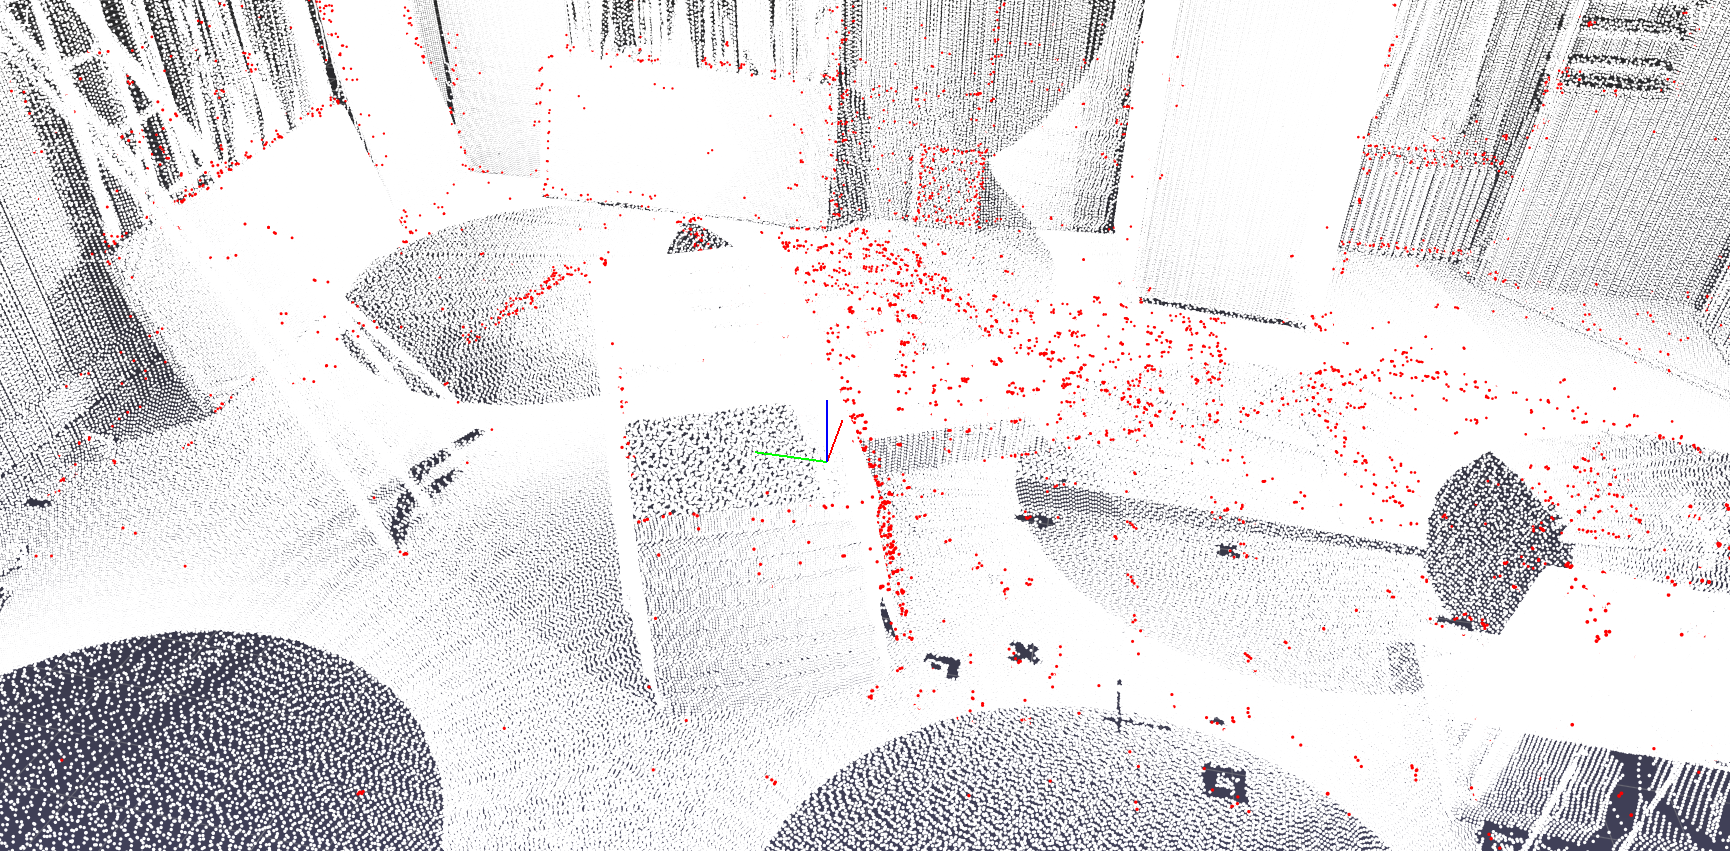
\includegraphics[width=3cm]{../masterthesis/img/pointcloud_orb} }}%
    \qquad
    \subfloat[\centering DSM]{{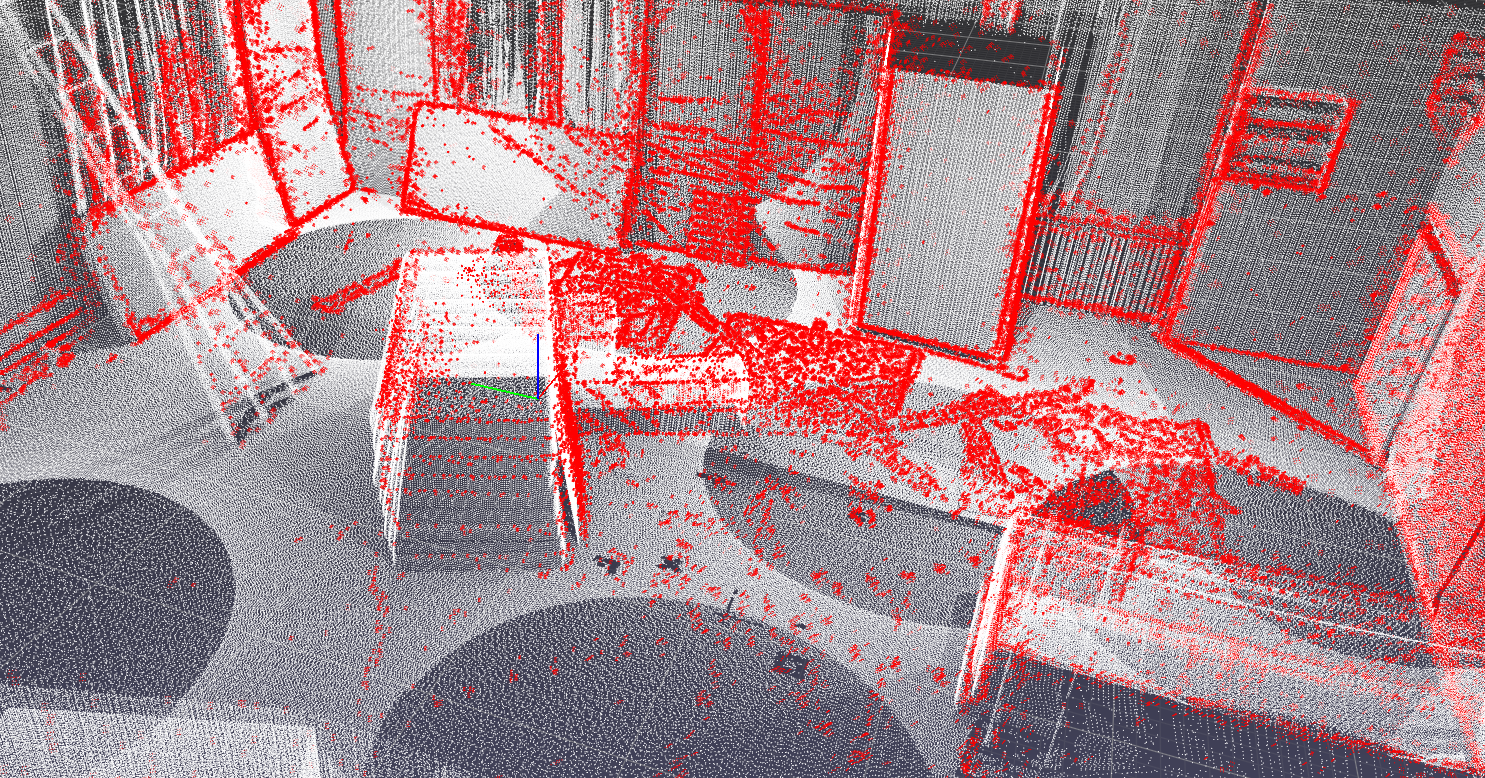
\includegraphics[width=3cm]{../masterthesis/img/pointcloud_dsm} }}%
	\qquad
    \subfloat[\centering DSO]{{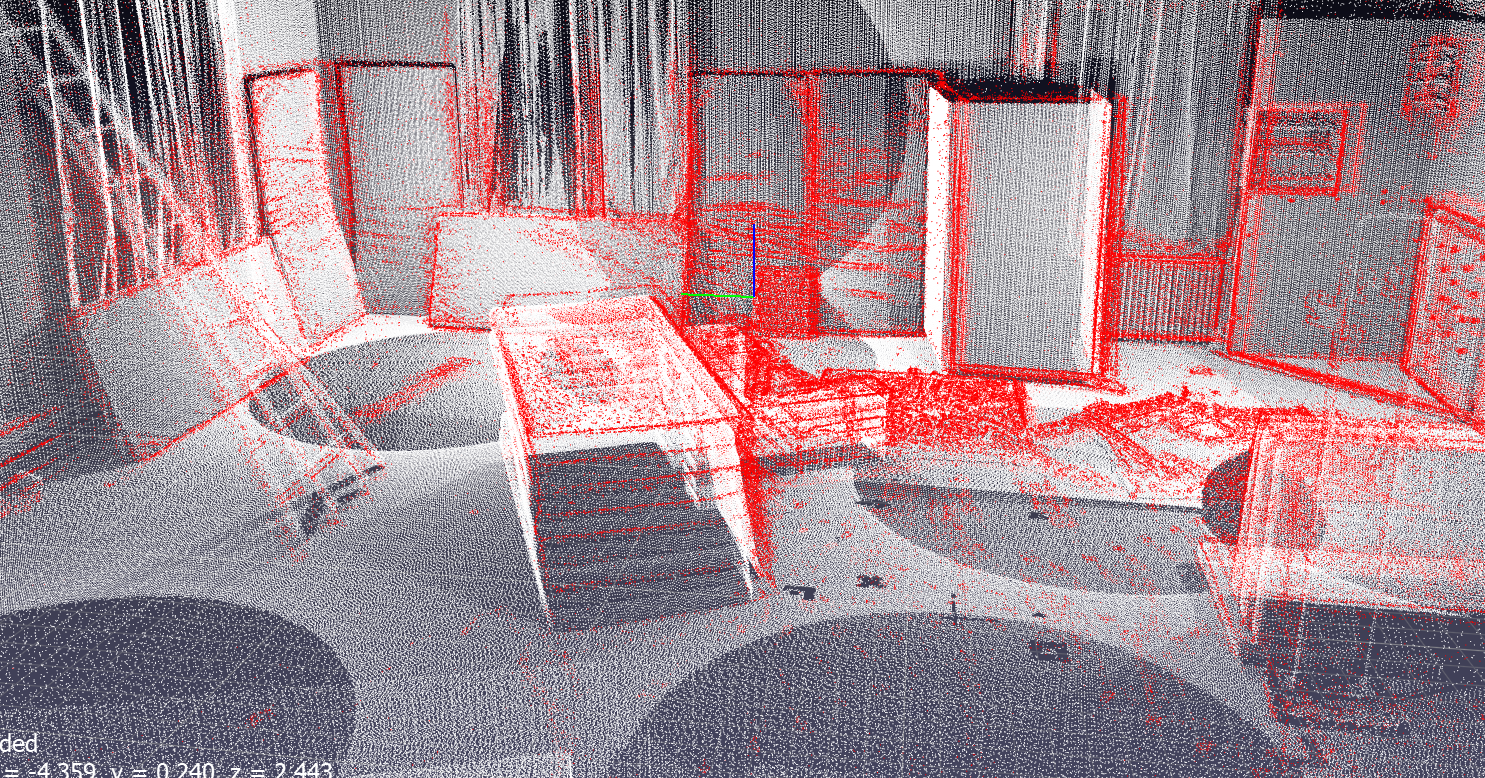
\includegraphics[width=3cm]{../masterthesis/img/pointcloud_dso} }}%
    \caption{The groundtruth of the Pointcloud from Sequence V101 (white points) and the evaluated points by each algorithm (red points). 
	The points in Figure (a) are four times as large for better visability (ORB-SLAM generates only few points). 
	}%
    \label{fig:pointcloud}%
\end{figure}


The computational effectiveness analysis expounded, that using the present setup, only ORB is capable of yielding a computational speed, that comes
close to real time. By downscaling the images, it was possible to 
run ORB on the sequences faster than realtime , without having major performance losses. 

This led to the conclusion that for the implementation of the whole 
autonomous system in ROS, ORB would be used as SLAM algorithm. This implementation has yet to be done. 


%
% ---- Bibliography ----
%
% BibTeX users should specify bibliography style 'splncs04'.
% References will then be sorted and formatted in the correct style.
%
% \bibliographystyle{splncs04}
% \bibliography{mybibliography}
%
\begin{thebibliography}{8}

\bibitem{point_cloud_eval}
J Wang et al.: Mapping quality evaluation of monocular slam solutions for micro aerial vehicals,2019

\bibitem{tasks}
Abhijeet Ravankar et al.: Autonomous Mapping and Exploration with
Unmanned Aerial Vehicles Using Low Cost Sensors, Hokkaido University 2018

\bibitem{point_cloud}
Nan Yang et al.: Feature-based or Direct: An Evaluation of Monocular Visual Odometry., Munich 2017.


\bibitem{ume}
Umeyama S., Least-Squares Estimation of Transformation Parameters Between Two Point Patterns, 1991


\end{thebibliography}
\end{document}